%! Author = jonathan
%! Date = 3/8/24

\section{Observations}\label{sec:observations}
Improving on the data report of related work~\cite{288705, 10.1145/3603269.3604869},
we use Nsight~\cite{nsys} to profile over 21k CUDA~\verb|All-to-All| kernels spanning three training runs of two
GPT-3 MoE models: 350M and 1.3B, on NDv2~\cite{azure} and 32 GPUs across 8 Perlmutter~\cite{perlm} nodes.
Note all experiments were performed on \emph{dedicated} hardware allocations without sharing.
\begin{figure}[!ht]
    \begin{subfigure}{.5\linewidth}
        \centering
        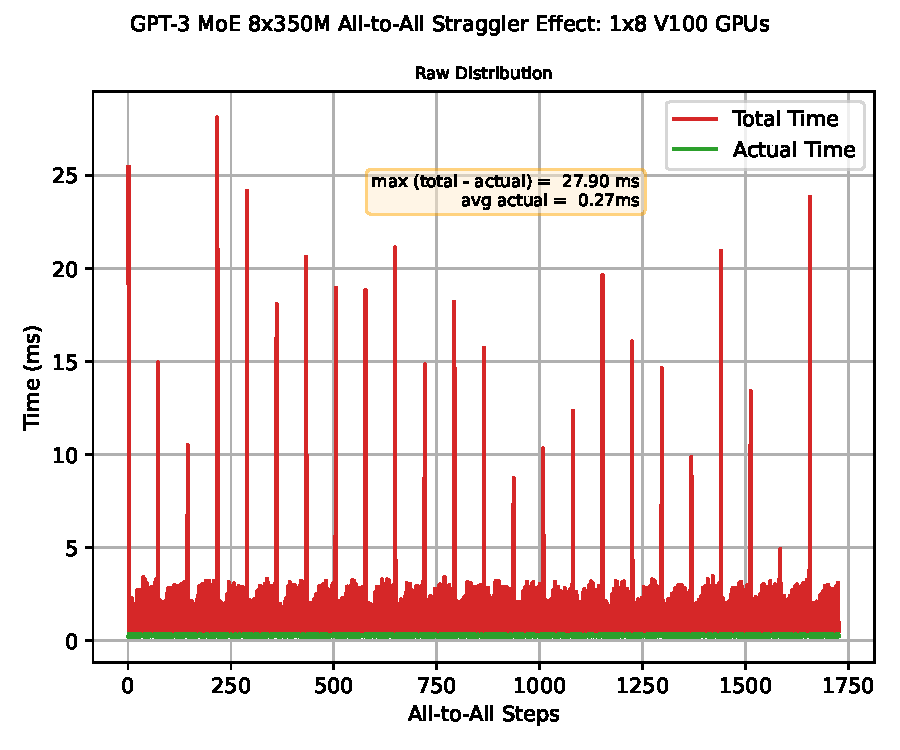
\includegraphics[width=0.8\linewidth]{images/GPT-3_MoE_8x350M}
        \caption{NDv2}
        \label{sub:s_350}
    \end{subfigure}\hfill % <-- "\hfill"
    \begin{subfigure}{.5\linewidth}
        \centering
        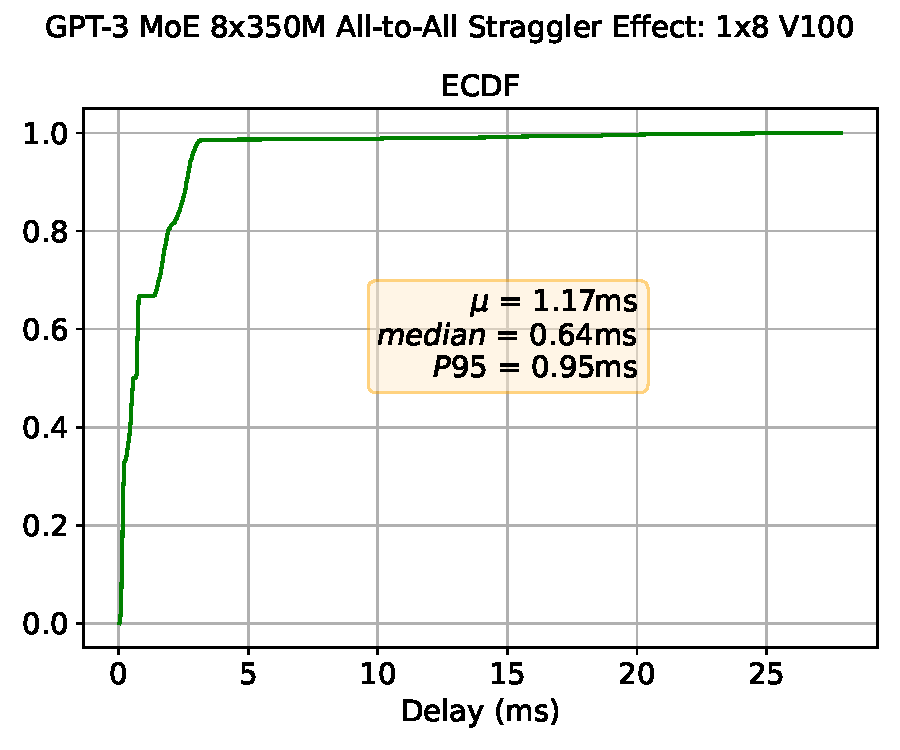
\includegraphics[width=0.8\linewidth]{images/GPT-3_MoE_8x350M_ecdf}
        \caption{NDv2 ECDF}
        \label{sub:s_350_ecdf}
    \end{subfigure}
    \medskip % create some *vertical* separation between the graphs
    \begin{subfigure}{.5\linewidth}
        \centering
        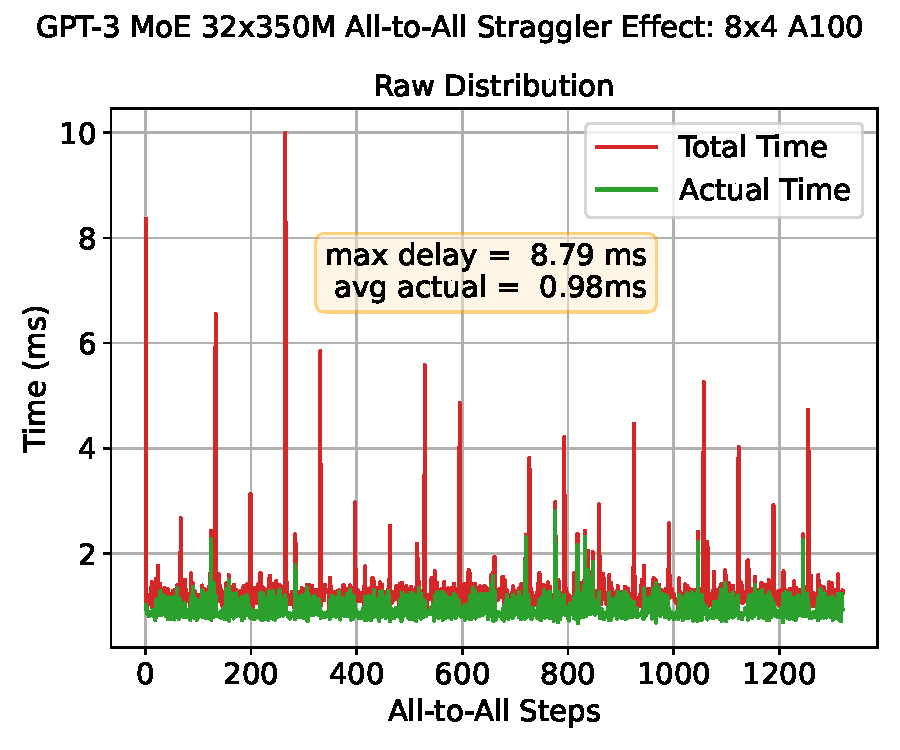
\includegraphics[width=0.8\linewidth]{images/GPT-3_MoE_32x350M}
        \caption{8x4 GPUs}
        \label{sub:m_350}
    \end{subfigure}\hfill % <-- "\hfill"
    \begin{subfigure}{.5\linewidth}
        \centering
        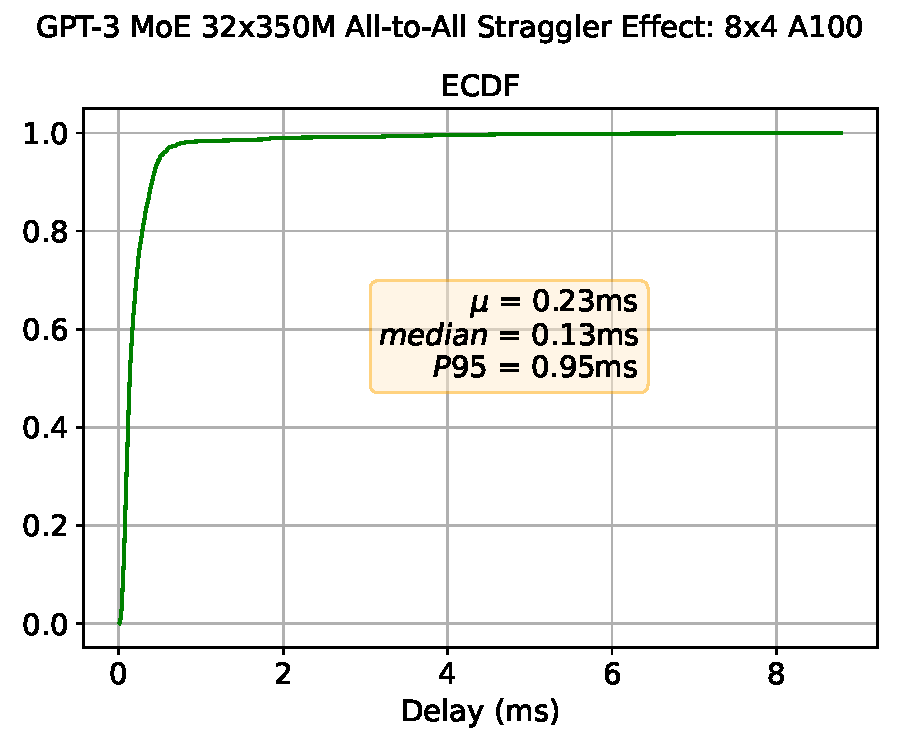
\includegraphics[width=0.8\linewidth, keepaspectratio]{images/GPT-3_MoE_32x350M_ecdf}
        \caption{8x4 GPUs ECDF}
        \label{sub:m_350_ecdf}
    \end{subfigure}
    \medskip % create some *vertical* separation between the graphs
    \begin{subfigure}{.5\linewidth}
        \centering
        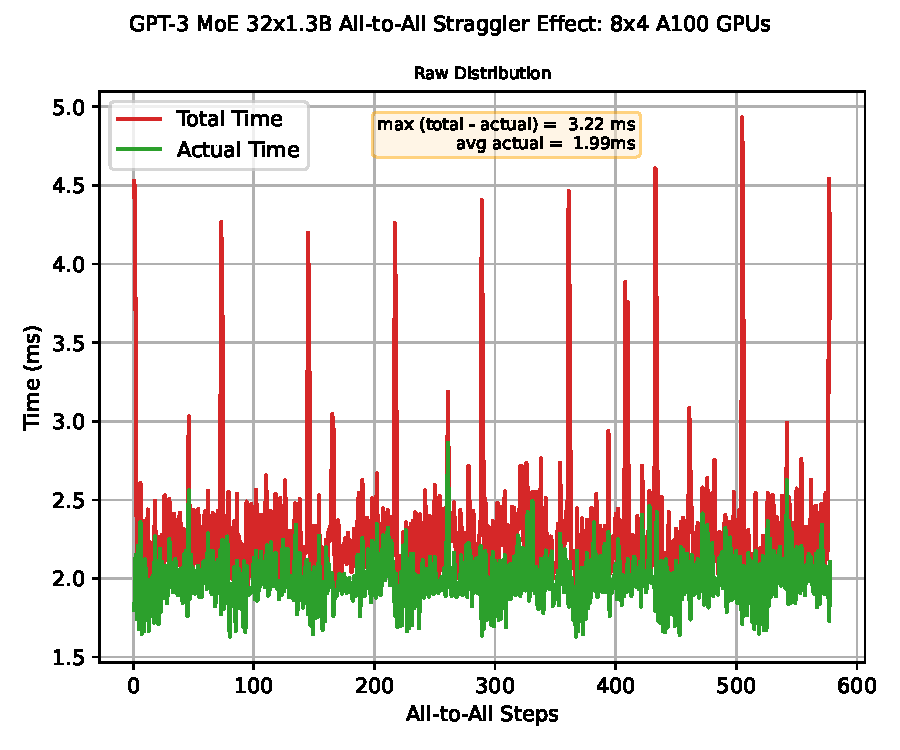
\includegraphics[width=0.8\linewidth]{images/GPT-3_MoE_32x1.3B}
        \caption{8x4 GPUs}
        \label{sub:m_1.3}
    \end{subfigure}\hfill % <-- "\hfill"
    \begin{subfigure}{.5\linewidth}
        \centering
        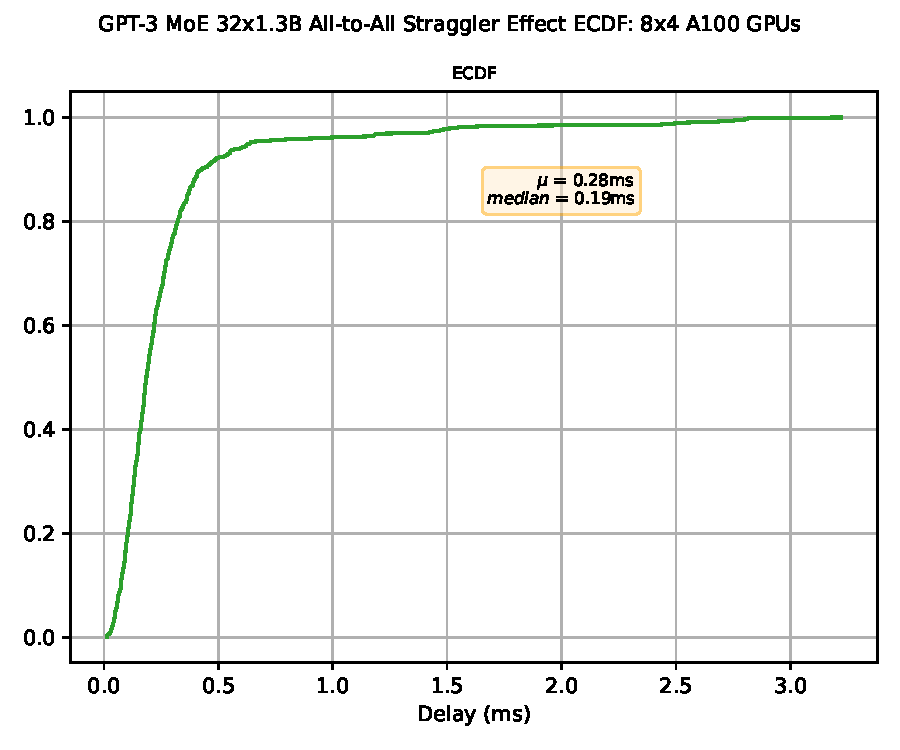
\includegraphics[width=0.8\linewidth, keepaspectratio]{images/GPT-3_MoE_32x1.3B_ecdf}
        \caption{8x4 GPUs ECDF}
        \label{sub:m_1.3_ecdf}
    \end{subfigure}
    \caption{\footnotesize Straggler Effect in DMoE Training.
    \textbf{Actual Time} $t_a$ denotes time for the slowest worker to complete the kernel,
        while \textbf{Total Time} $t$ includes time the fastest worker had to \emph{wait}. Note $Delay = t - t_a$}
    \label{fig:straggler}
\end{figure}

Figure~\ref{fig:straggler} makes it clear that the interconnect is not the bottleneck,
but rather the synchronization delay due to the implicit barrier of synchronous ~\verb|All-to-All|.
We clarify that the multi-node results should be much \emph{worse} on commodity clusters that do not
have the cluster-wide high-speed Slingshot-11~\cite{Khorassani2023} and RDMA software stack of the
Perlmutter supercomputer.
